%!TEX root = ../problems.tex
\begin{task}
	Найти спектр сигнала $S(t)=A\cdot \exp(-\frac{t^2}{\tau^2})$. Нарисовать график $|S(\omega)|$. Что будет при разных $\tau$?
\end{task}
\begin{proof}[\rm{\textbf{Решение}}]

\begin{equation}
	S(\omega)=A\newint \exp(-\frac{t^2}{\tau^2})e^{-i\omega t}\dd{t}
\end{equation}

Выделим полный квадрат в степени экспоненты. Схема выделения полного квадрата следующая. Пусть у нас есть выражение вида $a^2+b$, тогда можно привести его к виду полного квадрата следующим образом:
\begin{equation}
	a^2+b=a^2+2\cdot a \cdot d + d^2-d^2 = (a+d)^2-d^2
\end{equation}
Найти $d$ нетрудно: 
\begin{equation}
	d=\frac{b}{2a} \quad \Rightarrow \quad 
		a^2+b=\qty(a+\frac{b}{2a})^2-\frac{b^2}{4a^2}
\end{equation}
В нашем случае
\begin{equation}
	\frac{t^2}{\tau^2}+i\omega t=\qty(\frac{t}{\tau}+\frac{i\omega \tau}{2})^2-\qty(\frac{i\omega \tau}{2})^2
\end{equation}
И наш интеграл переходит в следующий:
\begin{equation}
	S(\omega)=A\exp(-\frac{\omega^2 \tau^2}{4})\newint \exp(\qty(\frac{t}{\tau}+\frac{i\omega \tau}{2})^2) \dd{t}
\end{equation}
Сделаем замену переменных: $\frac{t}{\tau}+\frac{i\omega \tau}{2} = x$ , $t=\tau x-\frac{i\omega \tau}{2}\tau$ , $dt=\tau dx$
\begin{equation}
	S(\omega)=A\tau \exp(-\frac{\omega^2 \tau^2}{4}) \newint e^{-x^2}dx
	=\qty(\,\newint e^{-x^2} dx=\sqrt\pi)=\sqrt\pi A\tau\cdot \exp(-\frac{\omega^2 \tau^2}{4})
\end{equation}

Найдем характерную временную ширину сигнала. Для экспоненциального спадения это время, за которое функция спадет в $e$ раз, и для нашей функции это время $\Delta t=\tau$.

Характерная ширина спектра находится анологично:
\begin{equation}
	\frac{\omega^2 \tau^2}{4}=1 \quad \Rightarrow \quad
		\Delta \omega=\frac{2}{\tau}
\end{equation}

Заметим отсюда характерное поведение спектра: чем уже сигнал во времени (меньше $\tau$), тем шире его частотный спектр.

\begin{figure}[h!]
	\centering
	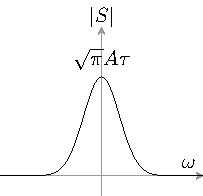
\includegraphics[scale=2.2]{ris/task1_out}
	\caption{Спектр сигнала}
	% \label{fig:figure1}
\end{figure}
\end{proof}